\label{sec:Rel4}

\begin{ejercicio} Calcule la recta que mejor aproxima por mínimos cuadrados discretos los datos $(-1,0)$, $\left(0, \frac{1}{2}\right)$, $(1,1)$, $(2,2)$ y $(3,2)$.
    \begin{equation*}
        \begin{array}{c|ccccc}
            x_i & -1 & 0 & 1 & 2 & 3 \\ \hline
            f(x_i) & 0 & \frac{1}{2} & 1 & 2 & 2
        \end{array}
    \end{equation*}
    
    Tenemos que $\bb{P}_1=\cc{L}\{1,x\}$. Por tanto, sea la recta buscada $L\equiv a_0+a_1x=0$. El producto escalar discreto empleado es:
    \begin{equation*}
        \langle f,g\rangle = \sum_{i=0}^4 f(x_i)g(x_i)
    \end{equation*}

    Calculo los productos escalares:
    \begin{gather*}
        \langle 1,1 \rangle = 5
        \qquad
        \langle 1,x \rangle = 5
        \qquad
        \langle x,x \rangle = 15
        \\
        \langle f,1\rangle = \frac{11}{2}
        \qquad
        \langle f,x \rangle = 11
    \end{gather*}

    Por tanto, el sistema a resolver, con la matriz de Gramm como matriz de coeficientes, es:
    \begin{equation*}
        \left(\begin{array}{cc}
            5 & 5 \\
            5 & 15
        \end{array}\right)
        \left(\begin{array}{c}
            a_0 \\ a_1    
        \end{array}\right)
        = 
        \left(\begin{array}{c}
            \frac{11}{2} \\ 11    
        \end{array}\right)
        \Longrightarrow
        \left\{\begin{array}{c}
            a_0 = \frac{11}{20} = 0.55  \\
            a_1 = \frac{11}{20} = 0.55
        \end{array}\right.
    \end{equation*}

    Por tanto, tenemos que la recta buscada mejor aproximación por mínimos cuadrados discretos de dichos datos es:
    \begin{equation*}
        L\equiv \frac{11}{20} + \frac{11}{20}x=0
    \end{equation*}

\end{ejercicio}


\begin{ejercicio}
    El dueño de un negocio en expansión observa que en los cinco primeros meses del año las ventas han sido de 40, 44, 52, 64 y 80 miles de euros, respectivamente.
    \begin{enumerate}
        \item Calcular la parábola de mínimos cuadrados $v(x) = a + bx + cx^2$ ($x$ = meses, $v(x)$ = ventas), resolviendo el sistema por el método de Gauss.
        \begin{equation*}
            \begin{array}{c|ccccc}
                x_i & 1 & 2 & 3 & 4 & 5 \\ \hline
                v(x_i) & 40 & 44 & 52 & 64 & 80
            \end{array}
        \end{equation*}

        Buscamos la mejor aproximación de dichos datos en $\bb{P}_2 = \cc{L}\{1,x,x^2\}$

        El producto escalar discreto empleado es:
        \begin{equation*}
            \langle f,g\rangle = \sum_{i=0}^4 f(x_i)g(x_i)
        \end{equation*}
    
        Calculo los productos escalares:
        \begin{gather*}
            \langle 1,1 \rangle = 5
            \qquad
            \langle 1,x \rangle = 15
            \qquad
            \langle 1,x^2 \rangle = 55
            \\
            \langle x,x^2 \rangle = 225
            \qquad
            \langle x,x \rangle = 55
            \qquad
            \langle x^2,x^2 \rangle = 979
            \\
            \langle f,1\rangle = 280
            \qquad
            \langle f,x \rangle = 940
            \qquad
            \langle f,x^2 \rangle = 3708
        \end{gather*}
    
        Por tanto, el sistema a resolver, con la matriz de Gramm como matriz de coeficientes, es:
        \begin{equation*}
            \left(\begin{array}{ccc}
                5 & 15 & 55\\
                15 & 55 & 225 \\
                55 & 225 & 979
            \end{array}\right)
            \left(\begin{array}{c}
                a \\ b \\ c    
            \end{array}\right)
            = 
            \left(\begin{array}{c}
                280 \\ 940  \\ 3708  
            \end{array}\right)
            \Longrightarrow
            \left\{\begin{array}{c}
                a = 40  \\
                b = -2 \\
                c=2
            \end{array}\right.
        \end{equation*}
    
        Por tanto, parábola $v$ buscada es:
        \begin{equation*}
            v(x)=40-2x+2x^2
        \end{equation*}

        \item Estime, según el modelo de ajuste anterior, las ventas que habrá a finales de año.

        Tenemos que las ventas en el último mes son de:
        \begin{equation*}
            v(12)=304 \text{ miles de euros}.
        \end{equation*}
    \end{enumerate}
\end{ejercicio}

\begin{ejercicio}
    Sea la función
    \begin{equation*}
        f(x)=\left\{\begin{array}{cc}
            0 & x\leq c \\
            2 & x>c
        \end{array}\right.
    \end{equation*}

    Sabemos que la recta que mejor aproxima a $f(x)$ por mínimos cuadrados continuos en el intervalo $[0, 3]$ es $\displaystyle p(x) = \frac{8}{9}x$. Calcule $c$.\\

    Al ser la aproximación por mínimos cuadrados continua en el intervalo $[0,3]$, tomamos el producto escalar:
    \begin{equation*}
        \langle f,g\rangle = \int_0^3 f(x)g(x)\;dx
    \end{equation*}

    Buscamos la mejor aproximación en $\bb{P}_1=\cc{L}\{1,x\}$. Calculamos los productos escalares:
    \begin{gather*}
        \langle 1,1\rangle = 3
        \qquad
        \langle 1,x\rangle = \frac{9}{2}
        \qquad
        \langle x,x\rangle = 9
        \\
        \langle f,1\rangle = \int_c^3 2\;dx = 2(3-c)
        \qquad
        \langle f,x\rangle = \int_c^3 2x\;dx = 9-c^2 
    \end{gather*}

    Por tanto, la mejor aproximación es $p(x)=a_0+a_1x \in \bb{P}_1$ tal que:
    \begin{equation*}
        \left(\begin{array}{cc}
            3 & 9/2 \\
            9/2 & 9
        \end{array}\right)
        \left(\begin{array}{c}
            a_0 \\ a_1    
        \end{array}\right)
        = 
        \left(\begin{array}{c}
            2(3-c) \\ 9-c^3
        \end{array}\right)
    \end{equation*}

    Como tenemos que la mejor aproximación es $p(x)=\frac{8}{9}x$, tenemos que $a_0=0$, $a_1=\frac{8}{9}$. Por tanto:
    \begin{equation*}
        \left\{\begin{array}{c}
            \displaystyle \frac{9}{2}\cdot \frac{8}{9} = 6-2c \Longrightarrow 4 = 6-2c  \\
            \\
            \displaystyle 9\cdot \frac{8}{9} = 9-c^3 \Longrightarrow 8=9-c^3
        \end{array}\right.
    \end{equation*}

    Por tanto, de ambas ecuaciones deducimos que $c=1$.
\end{ejercicio}



\begin{ejercicio} Sea $\omega : ]-1,1[\to \bb{R}$ dada por:
\begin{equation*}
    \omega(x) = 1 - x^2
\end{equation*}

    \begin{enumerate}
        \item Demuestre que la función $\omega(x) = 1 - x^2$ es una función peso en el intervalo $]-1,1[$.\\

        Tenemos que es integrable, ya que es una función continua con un dominio cerrado y acotado, por lo que su imagen es cerrada y acotada.

        Además, veamos que se cumple lo siguiente:
        \begin{equation*}
            \omega(x)\geq 0 \Longleftrightarrow
            1-x^2\geq 0
            \Longleftrightarrow
            1\geq x^2
            \Longleftrightarrow
            1\geq |x|
            \Longleftrightarrow -1 \leq x \leq 1
        \end{equation*}

        \item Utilizando el algoritmo de Gram–Schmidt, calcule una base ortogonal de $\bb{P}_2$ asociada al producto escalar continuo correspondiente a la función peso $\omega$ en el intervalo $]-1, 1[$.

        Tenemos que el producto escalar continuo es:
        \begin{equation*}
            \langle f,g \rangle = \int_{-1}^1 (1-x^2)f(x)g(x)\;dx
        \end{equation*}

        Tenemos que una base de $\bb{P}_2$ es $\cc{B}_u=\{1,x,x^2\}$ y sea la base ortogonal $\cc{B}_o=~\{e_1, e_2, e_3\}$. Partimos desde $e_1=1$.
        \begin{equation*}
            e_2 = x-\frac{\langle x,1\rangle}{\langle 1,1\rangle}\cdot 1 = x
        \end{equation*}
        \begin{equation*}
            \langle x,1\rangle = \int_{-1}^1(1-x^2)x\;dx = 0 \Longrightarrow x\perp 1
        \end{equation*}
        Por tanto, $e_2=x$. Calculamos ahora $e_3$.
        \begin{gather*}
            \langle x^2,1\rangle = \int_{-1}^1(1-x^2)x^2\;dx = \frac{4}{15}
            \qquad
            \langle 1,1\rangle = \int_{-1}^1(1-x^2)\;dx = \frac{4}{3}
            \\
            \langle x^2,x\rangle = \int_{-1}^1(1-x^2)x^3=0
        \end{gather*}
        \begin{equation*}
            e_3 = x^2 - \frac{\langle x^2,1\rangle}{\langle 1,1\rangle}e_1
            - \frac{\langle x^2,x\rangle}{\langle x,x\rangle}e_2
            = x^2 -\frac{3}{15}
        \end{equation*}

        Por tanto, tenemos que la base ortogonal de Gram-Schmidt es:
        \begin{equation*}
            \cc{B}_o = \left\{1,x,x^2 -\frac{3}{15}\right\}
        \end{equation*}

        \item Utilizando el apartado anterior, obtenga el polinomio de grado no mayor que 2 mejor aproximación por mínimos cuadrados de la función $f(x) = |x|$, con el producto escalar continuo correspondiente a la función peso $\omega$ en el intervalo $]-1, 1[$.\\

        Supongamos que la mejor aproximación es $p_2(x)\in \bb{P}_2$ de la forma $p_2(x)\equiv(a,b,c)_{\cc{B}_o} = a+bx +c\left(x^2-\frac{3}{15}\right)$.

        Calculamos, en primer lugar, los siguientes productos escalares:
        \begin{equation*}
            \langle f,1\rangle
            = \int_{-1}^1 (1-x^2)|x|\;dx
            = 2\cdot \int_{0}^1 x(1-x^2)\;dx
            = \frac{1}{2}
        \end{equation*}
        \begin{equation*}
            \langle f,x\rangle
            = \int_{-1}^1 (1-x^2)x|x|\;dx
            = 0
        \end{equation*}
        \begin{equation*}
            \left\langle f,x^2-\frac{3}{15}\right\rangle
            = \int_{-1}^1 (1-x^2)\left(x^2-\frac{3}{15}\right)|x|\;dx
            = 2\cdot\int_{0}^1 x^3(1-x^2)\;dx
            = \frac{1}{15}
        \end{equation*}

        Calculo además el cuadrado de cada elemento de la base ortogonal:
        \begin{gather*}
            \langle 1,1\rangle
            = \int_{-1}^1 (1-x^2)\;dx
            = \frac{4}{3}
            \qquad \qquad
            \langle x,x\rangle
            = \int_{-1}^1 x^2(1-x^2)\;dx
            = \frac{4}{15}
            \\
            \left\langle x^2 -\frac{3}{15},x^2 -\frac{3}{15}\right\rangle
            = \int_{-1}^1 \left(x^2 -\frac{3}{15}\right)^2 (1-x^2)\;dx
            = \frac{32}{525}
        \end{gather*}

        Por tanto, al haber elegido una base ortogonal, tenemos que:
        \begin{equation*}
            a = \frac{\langle f,1\rangle}{\langle 1,1\rangle} = \frac{1/2}{4/3} = \frac{3}{8}
            \qquad
            b = \frac{\langle f,x\rangle}{\langle x,x\rangle} = 0
            \qquad
            c = \frac{\left\langle f,x^2-\frac{3}{15}\right\rangle}{\left\langle x^2-\frac{3}{15},x^2-\frac{3}{15}\right\rangle} = \frac{1/15}{32/525} = \frac{35}{32}
        \end{equation*}

        Por tanto, tenemos que el polinomio buscado es:
        \begin{equation*}
            p_2(x)=\frac{3}{8} +\frac{35}{32}
            \left(x^2-\frac{3}{15}\right)
        \end{equation*}
        
    \end{enumerate}
\end{ejercicio}


\begin{ejercicio}\label{Ejercicio5}
    Determinar la recta que más se aproxima a la curva $f(x) = e^x$ según:
    \begin{enumerate}
        \item El método de mínimos cuadrados discreto en los puntos:
        \begin{equation*}
            -1\qquad -0.5 \qquad 0 \qquad0.5 \qquad1
        \end{equation*}

        Tenemos los siguientes nodos con sus respectivas imágenes:
        \begin{equation*}
            \begin{array}{c|ccccc}
                x_i & -1 & -0.5 & 0 & 0.5 & 1 \\ \hline
                e^{x_i} & \frac{1}{e} & \frac{1}{\sqrt{e}} & 1 & \sqrt{e} & e
            \end{array}
        \end{equation*}

        Tomamos como base de $\bb{P}_1$ $\cc{B}=\{1\}$. Sea por tanto la recta $r(x)=a_1 + a_2x$.

        El producto escalar discreto empleado es:
        \begin{equation*}
            \langle f,g\rangle = \sum_{i=0}^4 f(x_i)g(x_i)
        \end{equation*}
    
        Calculo los productos escalares:
        \begin{gather*}
            \langle 1,1\rangle = 5 \qquad
            \langle 1,x\rangle = 0 \qquad
            \langle x,x\rangle = \frac{5}{2}
            \\
            \langle f,1\rangle = \frac{e^2 + (e+1)(\sqrt{e}+1)}{e}
            \hspace{1cm}
            \langle f,x\rangle = \frac{2e^2 +\sqrt{e}(e-1)-2}{2e}
        \end{gather*}

        Por tanto, como tenemos que la base usada es ortogonal con este producto escalar, tenemos que:
        \begin{equation*}
            a_1 = \frac{\langle f,1\rangle}{\langle 1,1\rangle} = \frac{e^2 + (e+1)(\sqrt{e}+1)}{5e}
            \hspace{2cm}
            a_2 = \frac{\langle f,x\rangle}{\langle x,x\rangle} = \frac{2e^2 +\sqrt{e}(e-1)-2}{5e}
        \end{equation*}

        Por tanto, la recta mejor aproximación es:
        \begin{equation*}
            r(x)=\frac{e^2 + (e+1)(\sqrt{e}+1)}{5e} + \frac{2e^2 +\sqrt{e}(e-1)-2}{5e}x
        \end{equation*}
        
        
        \item El método de mínimos cuadrados continuo en $[-1, 1]$.
        
        Tomamos como base de $\bb{P}_1$ $\cc{B}=\{1\}$. Sea por tanto la recta $r(x)=a_1 + a_2x$.

        El producto escalar continuo empleado es:
        \begin{equation*}
            \langle f,g\rangle = \int_{-1}^1f(x)g(x)\;dx
        \end{equation*}
    
        Calculo los productos escalares:
        \begin{gather*}
            \langle 1,1\rangle = 2 \qquad
            \langle 1,x\rangle = 0 \qquad
            \langle x,x\rangle = \frac{2}{3}
            \\
            \langle f,1\rangle = \frac{e^2 -1}{e}
            \hspace{1cm}
            \langle f,x\rangle = \frac{2}{e}
        \end{gather*}

        Por tanto, como tenemos que la base usada es ortogonal con este producto escalar, tenemos que:
        \begin{equation*}
            a_1 = \frac{\langle f,1\rangle}{\langle 1,1\rangle} = \frac{e^2 -1}{2e}
            \hspace{2cm}
            a_2 = \frac{\langle f,x\rangle}{\langle x,x\rangle} = \frac{3}{e}
        \end{equation*}

        Por tanto, la recta mejor aproximación es:
        \begin{equation*}
            r(x)=\frac{e^2 -1}{2e} +  \frac{3}{e}x
        \end{equation*}
    \end{enumerate} 
\end{ejercicio}

\begin{ejercicio}
    Responda a los siguientes apartados:
    \begin{enumerate}
        \item Utilizando el algoritmo de Gram–Schmidt, calcule una base ortogonal de $\bb{P}_2$ utilizando el producto escalar discreto en los puntos $-1,\;0,\;1$, con pesos $1,\;2,\;1$, respectivamente.

        \begin{equation*}
            \begin{array}{c|ccc}
                x_i & -1 & 0 & 1 \\ \hline
                \omega(x_i) & 1 & 2 & 1
            \end{array}
        \end{equation*}

        Sea $\cc{B}_u=\{1,x,x^2\}$ base usual de $\bb{P}_2$, y buscamos una base ortogonal $\cc{B}_o=\{e_1, e_2, e_2\}$. Partimos de $e_1 = 1$, y empleando el algoritmo de Gram-Scmidt obtenemos el resto:
        \begin{equation*}
            e_2 = x - \frac{\langle x,e_1\rangle}{\langle e_1, e_1\rangle}\cdot e_1
        \end{equation*}

        El producto escalar discreto empleado es:
        \begin{equation*}
            \langle f,g\rangle = \sum_{i=1}^3 \omega(x_i)f(x_i)g(x_i)
        \end{equation*}

        Por tanto, el producto escalar necesario es:
        \begin{equation*}
            \langle x,1\rangle = -1+1=0
        \end{equation*}
        Por tanto, definimos $e_2=x$. Calculamos ahora $e_3$:
        \begin{equation*}
            e_3 = x^2 - \frac{\langle x^2,e_1\rangle}{\langle e_1, e_1\rangle}\cdot e_1 - \frac{\langle x^2,e_2\rangle}{\langle e_2, e_2\rangle}\cdot e_2
        \end{equation*}

        Calculo los productos escalares necesarios:
        \begin{equation*}
            \langle x^2,1\rangle = 1+1=2 \qquad
            \langle 1,1\rangle = 1+2+1=4 \qquad
            \langle x^2,x\rangle = -1+1=0
        \end{equation*}

        Por tanto,
        \begin{equation*}
            e_3 = x^2 - \frac{\langle x^2,e_1\rangle}{\langle e_1, e_1\rangle}\cdot e_1 - \cancelto{0}{\frac{\langle x^2,e_2\rangle}{\langle e_2, e_2\rangle}}\cdot e_2
            = x^2-\frac{2}{4} = x^2 - \frac{1}{2}
        \end{equation*}

        Por tanto, la base ortogonal es:
        \begin{equation*}
            \cc{B}_o = \left\{1,x,x^2-\frac{1}{2}\right\}
        \end{equation*}

        \item Obtenga el polinomio de grado no mayor que 2 mejor aproximación por mínimos cuadrados de la función
        $f(x) = x^{1/3}$ utilizando el apartado anterior.

        Sea el polinomio buscado $p(x)=a_1 + a_2x + a_3\left(x^2-\frac{1}{2}\right)$. Calculo los productos escalares necesarios para la matriz de Gram suponiendo el producto escalar del apartado anterior.
        \begin{gather*}
            \langle 1,1\rangle = 1+2+1=5 \qquad
            \langle x,x\rangle = 1+1=2 \qquad
            \\
            \langle 1,f\rangle = -1+0+1=0 \qquad
            \langle x,f\rangle = 1+0+1=2 \qquad
            \left\langle x^2-\frac{1}{2},f\right\rangle = -\frac{1}{2}+0+\frac{1}{2}=0 \qquad
        \end{gather*}

        Por trabajar con una base ortogonal, tenemos que:
        \begin{equation*}
            a_i = \frac{\langle e_i, f\rangle}{\langle e_i, e_i \rangle}
        \end{equation*}

        Por tanto, $a_1=a_3 = 0$, $a_2=1$. Es decir, la mejor aproximación en $\bb{P}_2$ es $p(x)=x$.
        \begin{observacion} Tenemos que la gráfica de $f(x)=x^{1/3}$ es la siguiente:
            \begin{figure}[H]
                \centering
                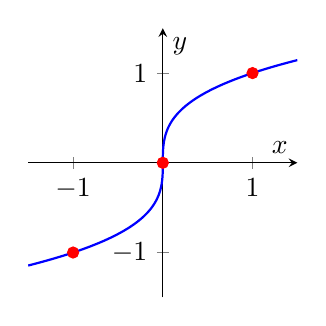
\begin{tikzpicture}
                \begin{axis}[
                    xlabel=$x$,
                    ylabel=$y$,
                    xmin=-1.5,
                    xmax=1.5,
                    ymin=-1.5,
                    ymax=1.5,
                    axis lines=middle,
                    width=5cm,
                    height=5cm,
                    samples=10000 %10000 % número de muestras para la función
                ]
                
                \addplot[blue, thick, domain=-1.5:1.5] {x^(1/3)};
                \addplot[blue, thick, domain=-1.5:1.5] {-(-x)^(1/3)};

                % Puntos marcados
                \addplot[red, only marks, mark=*] coordinates {(-1, {-(1)^(1/3)}) (0, {0^(1/3)}) (1, {1^(1/3)})};
    
                \end{axis}
                \end{tikzpicture}
            \end{figure}

            Como podemos ver, los tres puntos están alineados en la recta $y=x$, por lo que dicha recta los interpola y, por tanto, es la mejor aproximación a esos puntos.
        \end{observacion}
    \end{enumerate}
\end{ejercicio}

\begin{ejercicio}
    Obtenga la mejor aproximación de la función $f(x) = x^3$ mediante polinomios de segundo grado, con respecto a la medida combinada de distancia
    \begin{equation*}
        d(u,f)^2 = [u(0)-f(0)]^2 + \int_0^1 [u(x) - f(x)]^2\;dx
    \end{equation*}

    Calcule, además los tres primeros polinomios ortogonales asociados a este producto escalar.\\


    Tenemos que:
    \begin{equation*}
        d(u,f)^2 = \langle f-u,f-u\rangle = \langle u,u\rangle + \langle f,f\rangle -2\langle u,f\rangle
    \end{equation*}
    \begin{equation*}
        \begin{split}
            d(u,f)^2& = u^2(0) + f^2(0) -2u(0)f(0) + \int_0^1 u^2(x) + f^2(x) -2u(x)f(x)\;dx \\
            &= \left[u^2(0) + \int_0^1 u^2(x)\;dx\right] + \left[f^2(0) + \int_0^1 f^2(x)\;dx\right] -2\left[u(0)f(0) + \int_0^1 u(x)f(x)\;dx\right]
        \end{split}
    \end{equation*}

    Por tanto, por analogía de términos tenemos que el producto escalar empleado es:
    \begin{equation*}
        \langle f,g\rangle = f(0)g(0) -\int_0^1 f(x)g(x)\;dx
    \end{equation*}
\end{ejercicio}

\begin{ejercicio}
    Repita el ejercicio número \ref{Ejercicio5} utilizando el producto escalar continuo en el intervalo $[-1, 1]$, con peso $\omega(x) = x^2$. Es decir, determina la recta que más se aproxima a la curva $y = e^x$.
\end{ejercicio}

\begin{ejercicio}
    Calcule los polinomios de grados 1 y 2 que mejor aproximen por mínimos cuadrados discretos los datos de la siguiente tabla.
    \begin{equation*}
        \begin{array}{c|c|c|c|c|c}
            x_i & 4.0 & 4.2 & 4.5 & 4.7 & 5.1 \\ \hline
            y_i & 102.56 & 113.18 & 130.11 & 142.05 & 167.53
        \end{array}
    \end{equation*}
\end{ejercicio}

\begin{ejercicio}
    Se considera el producto escalar
    \begin{equation*}
        \langle f,g \rangle = \int_{-2}^{-1} f(x) g(x)\;dx + f(0) g(0) +\int_1^2f(x)g(x)\;dx.
    \end{equation*}

    \begin{enumerate}
        \item Calcule los tres primeros polinomios ortogonales.

        Consideramos el espacio vectorial $\bb{P}_n=\cc{L}\{1,x,x^2,\dots, x^n\}$ y buscamos una base ortogonal $\cc{B}_o = \{e_1, e_2, e_3, \dots, e_n\}$. Partimos de $e_1=1$, y usando el algoritmo de Gram-Schmidt, tenemos que:
        \begin{equation*}
            e_2 = x-\frac{\langle x, e_1\rangle}{\langle e_1, e_1\rangle} \cdot e_1
        \end{equation*}
        \begin{equation*}
            \langle x,1\rangle = \int_{-2}^{-1} x\;dx + 0 +\int_1^2 x\;dx = 0
        \end{equation*}

        Por tanto, definimos $e_2=x$. Calculamos ahora $e_3$
        \begin{equation*}
            e_3 = x^2-\frac{\langle x^2, e_1\rangle}{\langle e_1, e_1\rangle} \cdot e_1 -\frac{\langle x^2, e_2\rangle}{\langle e_2, e_2\rangle} \cdot e_2
        \end{equation*}
        \begin{equation*}
            \langle x^2,1\rangle = \int_{-2}^{-1} x^2\;dx + 0 +\int_1^2 x^2\;dx = \frac{14}{3}
            \qquad
            \langle x^2,x\rangle = \int_{-2}^{-1} x^3\;dx + 0 +\int_1^2 x^3\;dx = 0
        \end{equation*}
        \begin{equation*}
            \langle 1,1\rangle = \int_{-2}^{-1} 1\;dx + 1 +\int_1^2 1\;dx = 3
        \end{equation*}

        Por tanto, $e_3=x^2-\frac{14}{9}$. Es decir, los tres primeros polinomios ortogonales son:
        \begin{equation*}
            \left\{1,x,x^2-\frac{14}{9}\right\}
        \end{equation*}

        
        \item Utilizando el apartado anterior, proporcione la parábola $u(x)$ mejor aproximación por mínimos cuadrados de la función $f(x) = x^3$.

        Sea $\bb{P}_2=\cc{L}\left\{1,x,x^2-\frac{14}{9}\right\}$, y consideramos $u(x)=a_1 + a_2x + a_3\left(x^2-\frac{14}{9}\right)$.

        Calculamos productos escalares necesarios, sabiendo que se trata de una base ortogonal:
        \begin{equation*}
            \langle 1,1\rangle = 3 \qquad
            \langle x,x\rangle = \frac{14}{3} \qquad
            \langle x^2, x^2\rangle = \frac{62}{5}
        \end{equation*}
        \begin{equation*}
            \langle f,1\rangle = 0 \qquad
            \langle f,x\rangle = \frac{62}{5} \qquad
            \langle f, x^2\rangle = 0
        \end{equation*}

        Por trabajar con una base ortogonal, tenemos que:
        \begin{equation*}
            a_i = \frac{\langle e_i, f\rangle}{\langle e_i, e_i \rangle}
        \end{equation*}

        Por tanto, $a_1=a_3 = 0$. Además,
        \begin{equation*}
            a_2 = \frac{\langle x, f\rangle}{\langle x,x \rangle} = \frac{\frac{62}{5}}{\frac{14}{3}} = \frac{93}{35}
        \end{equation*}
        
        Es decir, la mejor aproximación en $\bb{P}_2$ es $$u(x)=\frac{93}{35}x$$
        
        \item Compruebe que $f(x) - u(x)$ es ortogonal a todos los polinomios de grado menor o igual a dos.

        Por ser $u$ la mejor aproximación de $f$, tenemos que:
        \begin{equation*}
            ||f-u||\leq ||f-p_2|| \Longrightarrow ||f-u||^2\leq ||f-p_2||^2 \qquad \forall p_2\in \bb{P}_2
        \end{equation*}

        Tomamos $g\in \bb{P}_2$, y sea $p_2=u+\lambda g \in \bb{P}_2 \mid \lambda \in \bb{R}$. Por tanto, como $p_2 \in \bb{P}_2$, tenemos que:
        \begin{equation*}
            ||f-u||^2\leq ||f-u-\lambda g||^2 = \langle f-u-\lambda g, f-u-\lambda g\rangle = ||f-u||^2 -2\lambda \langle f-u,g\rangle +\lambda^2 ||g||^2
        \end{equation*}

        Por tanto,
        \begin{equation*}
            0 \leq -2\lambda \langle f-u,g\rangle +\lambda^2 ||g||^2
            \qquad \forall \lambda\in \bb{R}, \forall g\in \bb{P}_2.
        \end{equation*}

        Considerando la expresión anterior como una parábola en la incógnita $\lambda$, tenemos:
        \begin{equation*}
            \Delta = 4(\langle f-u,g\rangle)^2 \geq 0
        \end{equation*}

        Por tanto, para que la parábola siempre sea positiva, no puede tener dos raíces. Por tanto, $\Delta=0$, lo que implica que:
        \begin{equation*}
            \langle f-u,g\rangle = 0 \qquad \forall g\in \bb{P}_2
        \end{equation*}

        Por tanto, hemos demostrado que $f(x) - u(x)$ es ortogonal a todos los polinomios de grado menor o igual a dos.
        
        \item Interprete geométricamente la distancia que induce este producto escalar.

        Tenemos que:
        \begin{equation*}
            d(u,v) := ||u-v||
            = \sqrt{\int_{-2}^{-1}(u-v)^2(x)\;dx + (u-v)^2(0) + \int_{1}^{2}(u-v)^2(x)\;dx}
        \end{equation*}

        Por tanto, la distancia es la raíz del área encerrada por ambas funciones entre $[-2, -1]$ y $[1,2]$ y el cuadrado de las imágenes de las dos funciones en $x=0$.

        Por tanto, al minimizar mediante mínimos cuadrados, lo que buscamos es minimizar el área entre dichas funciones en los intervalos mencionados y minimizar la distancia en el punto $x=0$.
        
        
        

        
    \end{enumerate}
\end{ejercicio}

\begin{ejercicio}
    Se considera la tabla de datos
    \begin{equation*}
        \begin{array}{c|c|c|c|c|c}
            x_i & -2 & -1 & 0 & 1 & 2 \\ \hline
            f(x_i)& -6.5 &-1.5 &-0.5& 3.5 &9.5
        \end{array}
    \end{equation*}


    \begin{enumerate}
        \item Calcule la aproximación por mínimos cuadrados de la función $f(x)$ en el espacio vectorial $\cc{U}=\cc{L}\{x,x^2\}$

        Sea la mejor aproximación $u(x)=ax + bx^2\in \cc{U}$, y consideramos el producto escalar discreto siguiente:
        \begin{equation*}
            \langle f,g\rangle = \sum_{i=1}^5 f(x_i)g(x_i)
        \end{equation*}

        Calculamos los siguientes productos escalares:
        \begin{equation*}
            \langle x,x\rangle = 10 \qquad \langle x^2, x^2\rangle = 34 \qquad \langle x,x^2\rangle = 0
        \end{equation*}
        \begin{equation*}
            \langle f,x\rangle = 37 \hspace{2cm} \langle f, x^2\rangle = 14
        \end{equation*}

        Por trabajar con una base ortogonal, tenemos que:
        \begin{equation*}
            a_i = \frac{\langle e_i, f\rangle}{\langle e_i, e_i \rangle}
        \end{equation*}

        Por tanto,
        \begin{equation*}
            a_1 = \frac{37}{10} \hspace{2cm} a_2 = \frac{14}{34} = \frac{7}{17}
        \end{equation*}

        Por tanto, la mejor aproximación de $f$ en $\cc{U}$ es:
        \begin{equation*}
            u(x) = \frac{37}{10}x + \frac{7}{17}x^2
        \end{equation*}
        

        \item Calcule las diferencias divididas de orden 1 (con dos argumentos) para los datos de la tabla y llámelas $P_1$, $P_2$, $P_3$ y $P_4$.
        \begin{gather*}
            P_1 = f[-2, -1] = \frac{-1.5+6.5}{-1+2} = 5
            \qquad
            P_2 = f[-1, 0] = 1
            \\
            P_3 = f[0,1] = 4
            \qquad
            P_4 = f[1,2] = 6
        \end{gather*}

        \item Calcule el spline cúbico de clase 1 en los nodos $-2$, $0$ y $2$, $s(x)\in S^1_3 (-2, 0, 2)$, tomando como derivadas en los nodos:
        \begin{equation*}
            d_0 = P_1,\qquad d_1=\frac{P_2+P_3}{2}, \qquad d_2=P_4.
        \end{equation*}

        Interpolamos mediante Hermite en cada intervalo:
        \begin{equation*}
            \begin{array}{c|cccc}
                &&\mathbf{[-2, 0]} \\ \\
                x_i & f(x_i) \\ \\
                -2 & \mathbf{-6.5} \\
                && \mathbf{d_0=5}\\
                -2 & -6.5 && \mathbf{-1}\\
                && 3 && \mathbf{\frac{3}{8}}\\ 
                0 & -0.5 && -\frac{1}{4}\\
                && d_1=\frac{5}{2}\\
                0 & -0.5
            \end{array}
            \quad \left\|\quad
            \begin{array}{c|cccc}
                &&\mathbf{[0,2]} \\ \\
                x_i & f(x_i) \\ \\
                0 & \mathbf{-0.5} \\
                && \mathbf{d_1=\frac{5}{2}}\\
                0 & -0.5 && \mathbf{\frac{5}{4}}\\
                && 5 && \mathbf{-\frac{3}{8}}\\ 
                2 & 9.5 && \frac{1}{2}\\
                && d_2=6\\
                2 & 9.5
            \end{array}\right.
        \end{equation*}
    
        Por tanto, el spline queda:
        \begin{equation*}
            s(x)=\left\{\begin{array}{lll}
                -6.5 +5(x+2) -(x+2)^2 +\frac{3}{8}x(x+2)^2 & \text{si} & x\in [-2, 0] \\
                -0.5+\frac{5}{2}x + \frac{5}{4}x^2 -\frac{3}{8}x^2(x-2) & \text{si} & x\in [0,2] \\
            \end{array} \right.
        \end{equation*}

        \item Compare los valores que proporcionan el spline y la aproximación por mínimos cuadrados en los nodos $-1$ y $1$. ¿Qué modelo elegiría?

        En $x=-1$, tenemos:
        \begin{equation*}
            s(-1)= -2.875 \hspace{2cm} u(-1)\approx -3.288
        \end{equation*}

        En $x=1$, tenemos:
        \begin{equation*}
            s(1)=3.625 \hspace{2cm} u(1)\approx 4.112
        \end{equation*}

        Por tanto, en ambos casos tenemos que el spline se aproxima más a los valores correctos de $f$.
    \end{enumerate}
\end{ejercicio}


\begin{ejercicio}
    La longitud de una varilla $L$ está ligada a la temperatura por el modelo lineal $L = a+bT$ . Calcula $a, b$ por mínimos cuadrados para los datos
    \begin{equation*}
        \begin{array}{c|c|c|c|c}
            T_i\;(^\circ C) & 20 & 40 & 50 & 60 \\ \hline
            L_i\;(mm.)&  1000.22 & 1000.65 & 1000.9 & 1001.05
        \end{array}
    \end{equation*}

    Se trata de una aproximación por mínimos cuadrados discreta en el espacio vectorial $\bb{P}_1[T] = \cc{L}\{1,T\}$.
\end{ejercicio}

\begin{ejercicio}
    La observación de un determinado proceso químico genera la tabla de datos siguiente
    \begin{equation*}
        \begin{array}{c|c|c|c|c|c}
            x_i & 1 & 1.2 & 1.5 & 1.7 & 2 \\ \hline
            y_i & 5 & 5.8 & 6.5 & 7.5 & 8.4
        \end{array}
    \end{equation*}

    \begin{enumerate}
        \item Determine la curva exponencial $y = ae^{bx}$ que ajusta dichos datos por el método de los mínimos cuadrados.

        Aplicando $\ln x$, tenemos que:
        \begin{equation*}
            \ln y = \ln (ae^{bx}) = \ln a + bx
        \end{equation*}

        Realizamos el cambio de variable $\ln y = y'$, $\ln a = a'$. Entonces, el problema se reduce a calcular la mejor aproximación $y'=a'+bx$ en $\bb{P}_1=\cc{L}\{1,x\}$.

        Consideramos el producto escalar discreto dado por:
        \begin{equation*}
            \langle f,g\rangle = \sum_{i=1}^5 f(x_i)g(x_i)
        \end{equation*}

        Calculamos los productos escalares necesarios:
        \begin{equation*}
            \langle 1,1\rangle = 5
            \qquad
            \langle x,x\rangle = 11.58
            \qquad
            \langle 1,x\rangle = 7.4
        \end{equation*}
        \begin{gather*}
            \langle y', 1\rangle = \sum_{i=1}^5 y'_i = \sum_{i=1}^5 \ln y_i = \ln\left(\prod_{i=1}^5 y_i\right) \approx 9.3822
            \\
            \langle y',x\rangle = \sum_{i=1}^5 x_iy'_i = \sum_{i=1}^5 x_i\ln y_i = \ln\left(\prod_{i=1}^5 (y_i)^{x_i}\right) \approx 14.2084
        \end{gather*}

        Por tanto, para calcular $a',b$ resolvemos el siguiente sistema:
        \begin{equation*}
            \left(\begin{array}{cc}
                5 & 7.4 \\
                7.4 & 11.58
            \end{array}\right)
            \left(\begin{array}{c}
                a' \\ b    
            \end{array}\right)
            = 
            \left(\begin{array}{c}
                9.3822 \\ 14.2084    
            \end{array}\right)
            \Longrightarrow
            \left\{\begin{array}{c}
                a' \approx 1.1158 \\
                b \approx 0.5139
            \end{array}\right.
        \end{equation*}

        Por tanto, tenemos que la mejor aproximación es:
        \begin{equation*}
            y' = a' +bx \Longrightarrow e^{y'} = e^{a'+bx} \Longrightarrow y=e^{a'}e^{bx} \approx 3.0521e^{0.5139x}
        \end{equation*}

        
        \item ¿Cuál es el valor esperado para $y$ cuando $x = 1.25$?

        Sustituyendo en la ecuación obtenida en el apartado anterior, tenemos que:
        \begin{equation*}
            y(x=1.25) = 5.802
        \end{equation*}
    \end{enumerate}
\end{ejercicio}

\begin{ejercicio}
    Sea $E = C([0, 1])$ dotado de su producto escalar usual y su norma asociada y sea $S$ el subespacio vectorial de $E$ tal que $S=\cc{L}\{1,x\}$. Dada $g \in E$, dada por $g(x) = x^2$ (con $0 \leq x \leq 1$), considera el problema de encontrar $h \in S$ de forma que $\displaystyle ||g - h|| = \min_{w\in S}{||g - w||}$. ¿Es unisolvente? ¿Por qué? En caso afirmativo, resuélvelo.

    Como las normas son no-negativas y $x^2$ es una función estrictamente creciente en $\bb{R}^+_0$, podemos elevar al cuadrado. Por tanto, buscamos $h\in S$ tal que:
    \begin{equation*}
        ||g - h||^2 = \min_{w\in S}{||g - w||^2}
    \end{equation*}

    Por definición de distancia, tenemos que buscamos $h\in S$ tal que:
    \begin{equation*}
        d^2(g, h) = \min_{w\in S}{d^2(g,w)}
    \end{equation*}

    Por tanto, tenemos que $h$ es la mejor aproximación de $g$ en $S=\bb{P}_1$. En este espacio vectorial, la mejor aproximación es única, por lo que nuestro problema es unisolvente.
\end{ejercicio}

\begin{ejercicio}
    Considere los datos
    \begin{equation*}
        (1,3), \qquad (1,-1), \qquad (e,2).
    \end{equation*}

    Determine razonadamente la curva de ecuación $y=\alpha\ln x + \beta$ que mejor los aproxima, en el sentido de los mínimos cuadrados.\\

    Realizamos un cambio de variable $x'=\ln x$:
    \begin{equation*}
        \begin{array}{c|c|c|c}
            x_i & 1 & 1 & e \\ \hline
            y_i & 3 & -1 & 2 \\ \hline
            x'=\ln x & 0 & 0 & 1
        \end{array}
    \end{equation*}

    Por tanto, el problema se reduce a ajustar $y=\alpha x' + \beta \in \bb{P}_1 = \cc{L}\{1,x'\}$.
    Consideramos el producto escalar discreto dado por:
    \begin{equation*}
        \langle f,g\rangle = \sum_{i=1}^3 f(x_i)g(x_i)
    \end{equation*}

    Como dos valores de las abscisas son iguales, tenemos que no es un producto escalar en $\bb{P}_3$ ni en $\bb{P}_2$. No obstante, sí lo es $\bb{P}_1$, que es el espacio vectorial que nos concierne.

    Calculamos los productos escalares necesarios:
    \begin{equation*}
        \langle 1,1\rangle = 3
        \qquad
        \langle x',x'\rangle = 1
        \qquad
        \langle 1,x'\rangle = 1
    \end{equation*}
    \begin{equation*}
        \langle y, 1\rangle = 4
        \quad
        \langle y,x'\rangle = 2
    \end{equation*}

    Por tanto, para calcular $a',b$ resolvemos el siguiente sistema:
    \begin{equation*}
        \left(\begin{array}{cc}
            3 & 1 \\
            1 & 1
        \end{array}\right)
        \left(\begin{array}{c}
            \beta \\ \alpha    
        \end{array}\right)
        = 
        \left(\begin{array}{c}
            4 \\ 2    
        \end{array}\right)
        \Longrightarrow
        \left\{\begin{array}{c}
            \alpha = 1 \\
            \beta = 1
        \end{array}\right.
    \end{equation*}

    Por tanto, tenemos que la mejor aproximación es:
    \begin{equation*}
        y = x' +1 \Longrightarrow y = \ln x +1
    \end{equation*}
    
\end{ejercicio}

\end{document}